\paragraph{\textit{The Nash Equilibrium.}}
The Nash equilibrium of our Baseline Game depends on the the first component of the payoff function. The following table presents individual payoff at each round of extraction decision. The payoff matrix presented in Table \ref{tab:5} represents the strategies and payoffs each participant will receive in terms of 2 players setting. By iterated elimination, we can see that extracting 7 trees at every round is the dominant strategy where neither players no longer have incentives to deviate. Although the matrix depicts a game with 2 players, since the game is symmetric, the payoffs for playing a particular strategy depend only on the other strategies employed, and not on who is playing them. From here we can deduce that the third player in the group will want to take the same dominant strategy, knowing that the other two players' best response is to also harvest 7 trees. Consequently, the third player's best response to the dominant strategy of the other 2 players will be also to harvest 7 trees at any given round.


\begin{table}[h]
  \centering
  \caption{Players Payoff Matrix}\label{tab:5}
  \begin{tabular}{l|c|c|c|c|c|c|c|c|c}
    \toprule
    \multicolumn{2}{c}{} &\multicolumn{7}{c}{P2/P3} \\ \cline{3-10}
    \multicolumn{2}{c}{}    & 7 & 6 & 5 & 4 & 3 & 2 & 1 & 0 \\ \hline \hline
    \multirow{8}{*}{P1} & 7 & \textbf{(14,14)} & \sout{(14,12)} & \sout{(14,10)} & \sout{(14,8)} & \sout{(14,6)} & \sout{(14,4)} & \sout{(14,2)} & \sout{(14,0)} \\ \cline{2-10}
                        & 6 & \sout{(12,14)} & \sout{(12,12)} & \sout{(12,10)} & \sout{(12,8)} & \sout{(12,6)} & \sout{(12,4)} & \sout{(12,2)} & \sout{(12,0)} \\ \cline{2-10}
                        & 5 & \sout{(10,14)} & \sout{(10,12)} & \sout{(10,10)} & \sout{(10,8)} & \sout{(10,6)} & \sout{(10,4)} & \sout{(10,2)} & \sout{(10,0)} \\ \cline{2-10}
                        & 4 & \sout{(8,14)} & \sout{(8,12)} & \sout{(8,10)} & \sout{(8,8)} & \sout{(8,6)} & \sout{(8,4)} & \sout{(8,2)} & \sout{(8,0)} \\ \cline{2-10}
                        & 3 & \sout{(6,14)} & \sout{(6,12)} & \sout{(6,10)} & \sout{(6,8)} & \sout{(6,6)} & \sout{(6,4)} & \sout{(6,2)} & \sout{(6,0)} \\ \cline{2-10}
                        & 2 & \sout{(4,14)} & \sout{(4,12)} & \sout{(4,10)} & \sout{(4,8)} & \sout{(4,6)} & \sout{(4,4)} & \sout{(4,2)} & \sout{(4,0)} \\ \cline{2-10}
                        & 1 & \sout{(2,14)} & \sout{(2,12)} & \sout{(2,10)} & \sout{(2,8)} & \sout{(2,6)} & \sout{(2,4)} & \sout{(2,2)} & \sout{(2,0)} \\ \cline{2-10}
                        & 0 & \sout{(0,14)} & \sout{(0,12)} & \sout{(0,10)} & \sout{(0,8)} & \sout{(0,6)} & \sout{(0,4)} & \sout{(0,2)} & \sout{(0,0)} \\ \cline{2-10}
    \bottomrule
  \end{tabular}
\end{table}


\noindent Given that harvesting 7 trees in any given round is the dominant strategy of every player due to the symmetry of the game, then it must also follow that all members of the group to play this dominant strategy is the Nash equilibrium. This is because, in a Nash equilibrium, no player can benefit by unilaterally changing their strategy, given the strategies of the other players. Since a dominant strategy is the best response to any strategy of the opponents, once players choose their dominant strategies, no one has an incentive to deviate.

\begin{figure}[H]
  \centering
  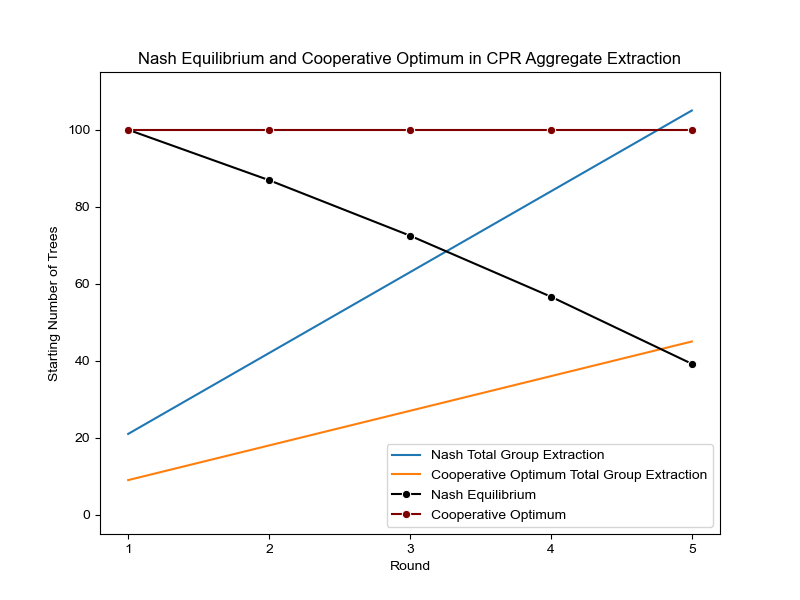
\includegraphics[width=0.7\linewidth]{../bld/graphs/0.Nash&Cooperative Baseline.png}
  \caption{Nash Equilibrium and Cooperative Equilibrium}\label{fig:nash&cooperative}
\end{figure}

 From this, we can expect that a fully rational and selfish player will always thrive to harvest seven trees at every round regardless of the other group members' decision. Harvesting seven trees in every round is also the Nash equilibrium since extracting seven trees provide no other incentive for any group member to deviate. From the Nash equilibrium, we can also expect that a selfish group that strive to maximize only his or her personal payoff from harvesting, will always harvest 21 trees in total in every round which consequently will drop resource stock faster than the alternatives as depicted in Figure \ref{fig:nash&cooperative}.


\paragraph{\textit{The Cooperative Solution Maximizes Social Payoff.}}
In contrast to Nash equilibrium, the optimum payoff for society - which we call the Cooperative Solution - is for everyone in the group to harvest only three trees in any given round. To see this, the number of trees in the forest is bounded between zero and 100 ($0\leq Z \leq 100$). With backward induction to determine the optimal social payoff, we can quickly deduct that $Z_5=100$ is the number of trees that maximizes the total expected payoff for the group as a whole. In order to achieve $Z_5=100$, the Cooperative solution is for every member of the group to harvest only three trees in any given round, noting further that everyone in the group always play the same strategy.

\paragraph{Cooperative Solution Calculation}
 To see this, the number of trees in the forest is bounded between 0 and 100 ($0\leq Z \leq 100$). With backward induction to determine the optimal social payoff, we can quickly deduct that $Z_5=100$ is the number of trees that maximizes the total expected payoff of for the group as a whole. In order to achieve $Z_5=100$, with regrowth rate of $10\%$ we know that there should be 90.9 trees left in the forest after extraction. Consequently, to have at least 90.9 trees after extraction requires that $Z_4$, the remaining trees in round 4, should also be 100. Thus,
\begin{align*}
    Z_5 &= (Z_4 - X_5)1.1 \\
    100 &= (100 - X_5)1.1 \\
    90.9 &= 100 - X_5 \\
    X_5 &= 9.1 \\
\end{align*}
In round 5, the group as whole must only extract maximum of 9.1 trees in total to maintain the maximum forest capacity. Provided that
\begin{align*}
    X_{t} &= \sum_{i=1}^{3} x_{i,t} \\
    9.1 &= \sum_{i=1}^{3} x_{i,t} \\
    x_{i,t} &= 3.0\dot{3}
\end{align*}
The same logic then applies for the previous rounds, resulting in each individual to cut maximum 3 trees. Thus, the maximum number of trees that maximizes social payoff can be achieved if and only if every member of the group to harvest 3 trees or less in any given round. However, individuals can only maximize their payoff while maintaining social optimum if and only if they harvest precisely 3 trees in all rounds.

 Provided that harvesting seven trees in every round is the dominant strategy in the game, maintaining Cooperative Equilibrium is difficult. The difficulties are two folds; firstly the Cooperative equilibrium is unstable. Maintaining one or everyone to harvest only three trees is difficult because taking more than three trees provides players higher payoff, and hence, there are incentives to deviate. Secondly, cooperation through communication is impossible during the game since members in a group do not know who their team members are, and they were not allowed to communicate with other players throughout the game. Thus, for a player or all players in a group to choose three trees in each round must be out of altruistic behaviour, i.e, a strategy that aims to achieve the socially optimal solution even though it might be at the expense of oneself.

%\paragraph{\textit{The trade-off between efficiency and self maximizing strategies.}}
 Going back to individual players' and group payoff function, notice that the first component in the payoff function described in equation \ref{eq:2} is monotonic in nature. The higher the number of trees harvested by any players proportionately increases their payoffs. This first component is what drives our Nash equilibrium which selfish and fully rational behaviour will maximize the individual payoff. However, the higher the number of trees extracted by individual consequently reduces the remaining number of trees available aggregately as a group as defined in equation \ref{eq:1}. Notice that the second component in our payoff function depends on $Z_5$ where $Z_5$ is a $5^{th}$ degree polynomial function that optimizes social payoff when all players symmetrically harvest three trees at all rounds. This concave function defines the choice between increasing own payoff at the expense of efficiency for society, which is precisely the trade-off that individual and a group will have to make in the game.

 To show the trade-off between individual's own payoff and the socially desirable choice, let's take the Pareto optimal solution, where each member of the group extracts three trees in each round. In this case, the total payoff will be maximized. However, each individual has the choice to deviate from the equilibrium by extracting more trees. Any unilateral deviations increases the individual's payoff. Therefore we can say that by extracting marginally more trees ceteris paribus, the agent increases her own payoff but decreases the total social payoff. In other words, he or she faces a trade-off between socially desirable behaviour and selfishness. In contrast, take for example the case when a player extracts less than three trees. To deviate from the socially desirable choice on the surface may seem to be contradictive or even foolish. However, the fact that the Pareto optimum is unstable makes such choice understandable to even occur. If one player expects the other two players to be selfish (harvesting more than three trees) yet she cares more about the social payoff than about her own payoff, she cuts less trees then the socially desired choice. In other words, this player faces a trade-off between achieving a more socially desirable outcome and maximizing her own payoff.

\begin{figure}[H]
  \centering
  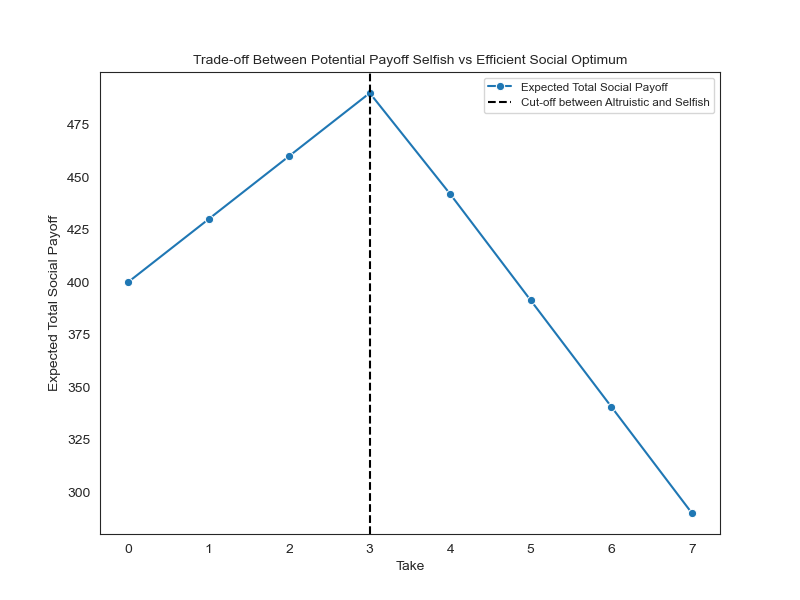
\includegraphics[width=0.6\linewidth]{../bld/graphs/0.Tradeoff1.png}
  \caption{Trade-off Between Potential Payoff Selfish vs Efficient Social Optimum}\label{fig:tradeoff2}
\end{figure}
 Figure\ref{fig:tradeoff2} depict this trade-off. Notice that even though harvesting three or less gives higher potential payoff to society compared to selfish behaviour, individuals can still make themselves better off by choosing precisely three trees instead of anything less. The peak potential payoff to society lies exactly at the point where harvesting three trees is the strategy adopted by all members of the group. Anything less or above this point is no longer the optimal point, and thus, a trade-off exists.

\paragraph{\textit{Individual Behaviour Type.}}
Since each member of the group makes five choices, it would be interesting to see how their behavior change from round to round as a response to when they learn the type of their group members (either altruistic, socially desirable or selfish). For example, if all players chose to play the dominant strategy, then the Nash equilibrium will prevail whereby individuals care only about maximizing his or her own payoff at the expense of society. On the contrary, if all individuals refrain from harvesting more than three trees per round, the expected total social payoff as a group will be much higher than in the Nash equilibrium.

 Provided this trade-off, harvesting 3 trees in any given round is the socially optimum behaviour that individuals can do. Whereas any other strategies to the left of this social optimum in figure \ref{fig:tradeoff2}, we will call this \textit{pro-environmental behaviour} by which individual altruistically chooses to harvest number of trees that benefits society at the expense of oneself. Similarly, any other action to the right of the socially maximizing strategy, we name them \textit{selfish behaviour} by which individuals care only of one's payoff at the expense of society.



%add gametheoretical, game expected results
% study design, experminetal procedure, behavioural prediction (check consecutive order) *
% design were pre-registered before and approval ethics gfeb
